\documentclass[11pt]{article}

\usepackage[margin=1in]{geometry}
\usepackage{amsmath}
\usepackage{graphicx}
\usepackage{float}

\title{RL Lab 1 -- Exploration vs Exploitation}
\author{Fotios Kapotos}
\date{}

\begin{document}

\maketitle

\section{RL Lab 1 -- Exploration vs Exploitation}

\subsection{Greedy Agent}

\subsubsection{How did our agent do?}

The greedy agent performs well at the beginning by quickly exploiting the action that appears to give the highest reward. However, its performance soon plateaus at a suboptimal level. Because the agent never explores, it can commit early to a suboptimal action due to noisy initial rewards and is unable to recover. Its long-term performance is therefore limited.

\begin{figure}[h]
    \centering
    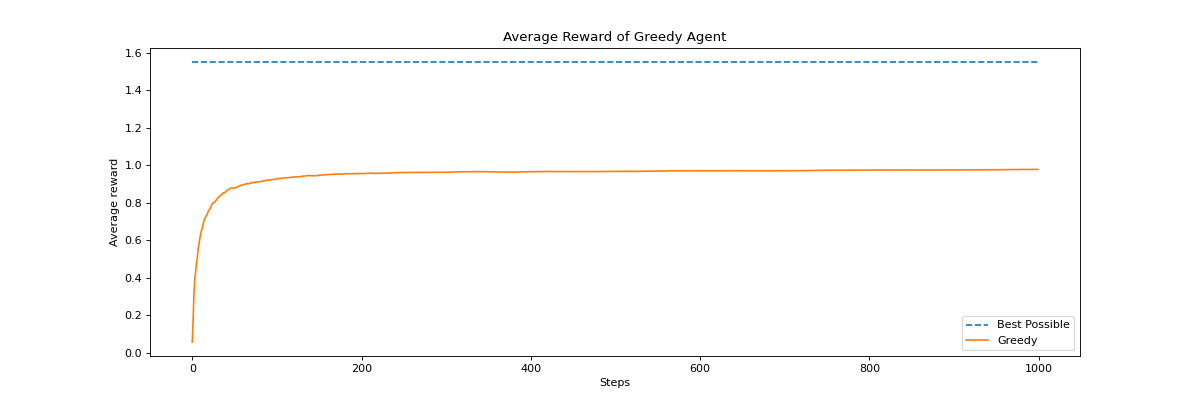
\includegraphics[width=0.85\linewidth]{../figures/greedy.png}
    \caption{Average reward over time for the greedy agent.}
\end{figure}

\subsection{Epsilon-Greedy Agent}

\subsubsection{What do you notice?}

Compared to the greedy agent, the $\epsilon$-greedy agent initially performs slightly worse due to exploration (see Figure~\ref{fig:epsilon-greedy}). However, over time it achieves a higher average reward. By occasionally exploring, the agent is able to correct early estimation errors and identify the true optimal action, leading to better long-term performance.

\begin{figure}[h]
    \centering
    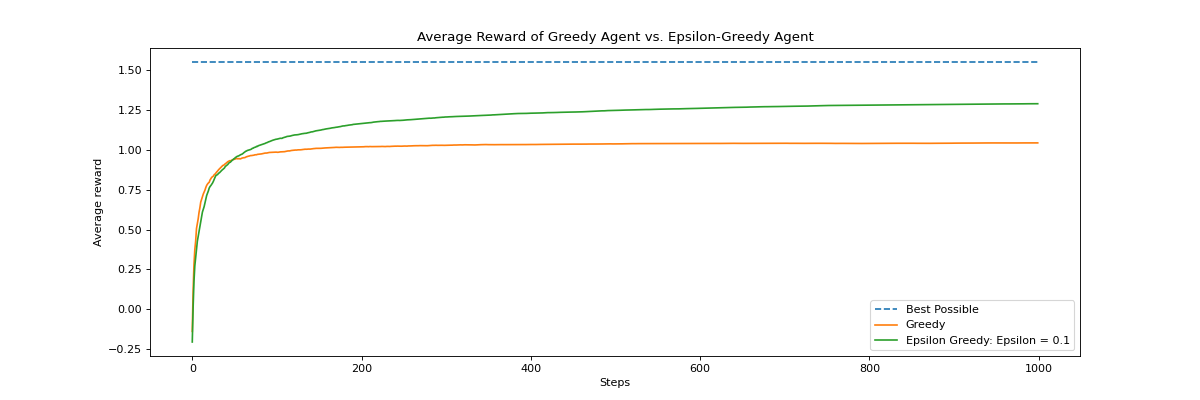
\includegraphics[width=0.85\linewidth]{../figures/epsilon-greedy.png}
    \caption{Average reward over time for the $\epsilon$-greedy and the greedy agent.}
    \label{fig:epsilon-greedy}
\end{figure}
\subsection{Comparing Values of $\epsilon$}

\subsubsection{Why did $\epsilon = 0.1$ perform better than $\epsilon = 0.01$?}

With $\epsilon = 0.1$, the agent explores frequently enough to reliably discover the optimal action and update its value estimates. In contrast, $\epsilon = 0.01$ behaves almost greedily and explores too rarely, making it more likely to get stuck exploiting a suboptimal action discovered early.

\begin{figure}[h]
    \centering
    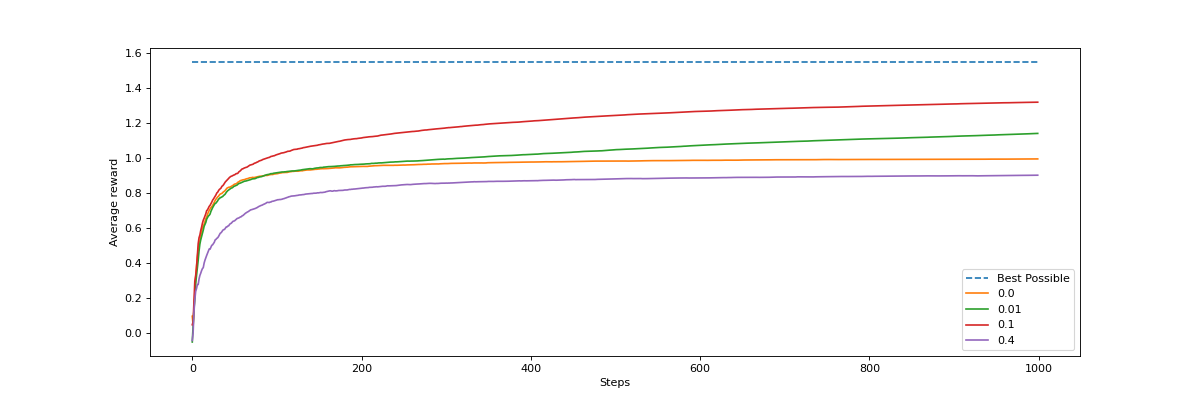
\includegraphics[width=0.85\linewidth]{../figures/epsilons.png}
    \caption{Comparison of average reward for $\epsilon = 0.1$, $\epsilon = 0.01$, $\epsilon = 0.4$ and greedy}
\end{figure}

\subsubsection{Why did $\epsilon = 0.4$ perform worse than $\epsilon = 0.0$ (the greedy agent)?}

With $\epsilon = 0.4$, the agent explores excessively, selecting random actions a large fraction of the time. This prevents sufficient exploitation of high-reward actions, resulting in a lower average reward than the greedy agent, which consistently exploits its best-known action.

\subsection{Effects of the Step Size}

\subsubsection{Effect of $\alpha = 1 / N(A)$}

The agent using a step size of $\alpha = 1 / N(A)$ performs well early on because initial updates are large and learning is fast. However, as $N(A)$ increases, the step size shrinks toward zero. When the environment changes, new rewards have little influence on the value estimates, preventing the agent from adapting and causing its performance to degrade.

\begin{figure}[h]
    \centering
    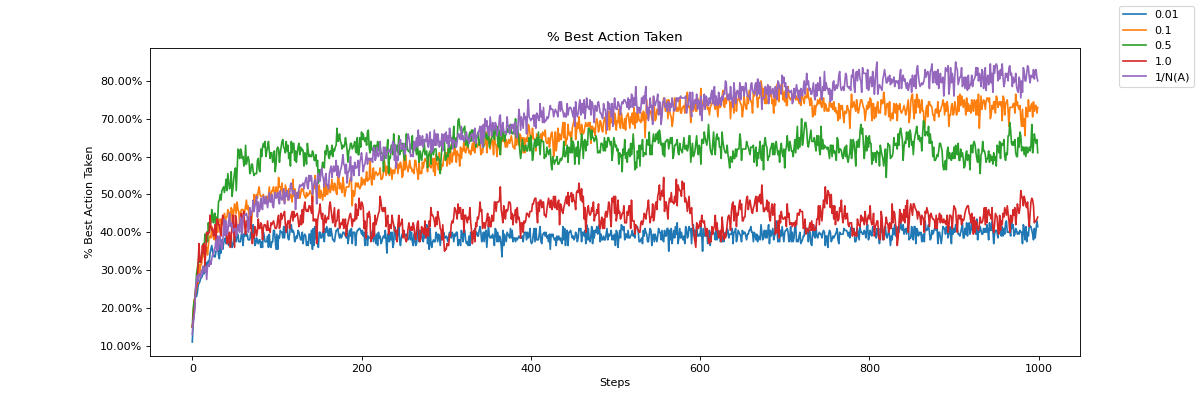
\includegraphics[width=0.85\linewidth]{../figures/N evolution.png}
    \caption{Effect of step size on performance in a non-stationary environment.}
\end{figure}

\end{document}